\section{ИССЛЕДОВАНИЕ РАБОТЫ РЕВЕРСИВНОГО СЧЕТЧИКА}


\begin{figure}[H]
	\centering
	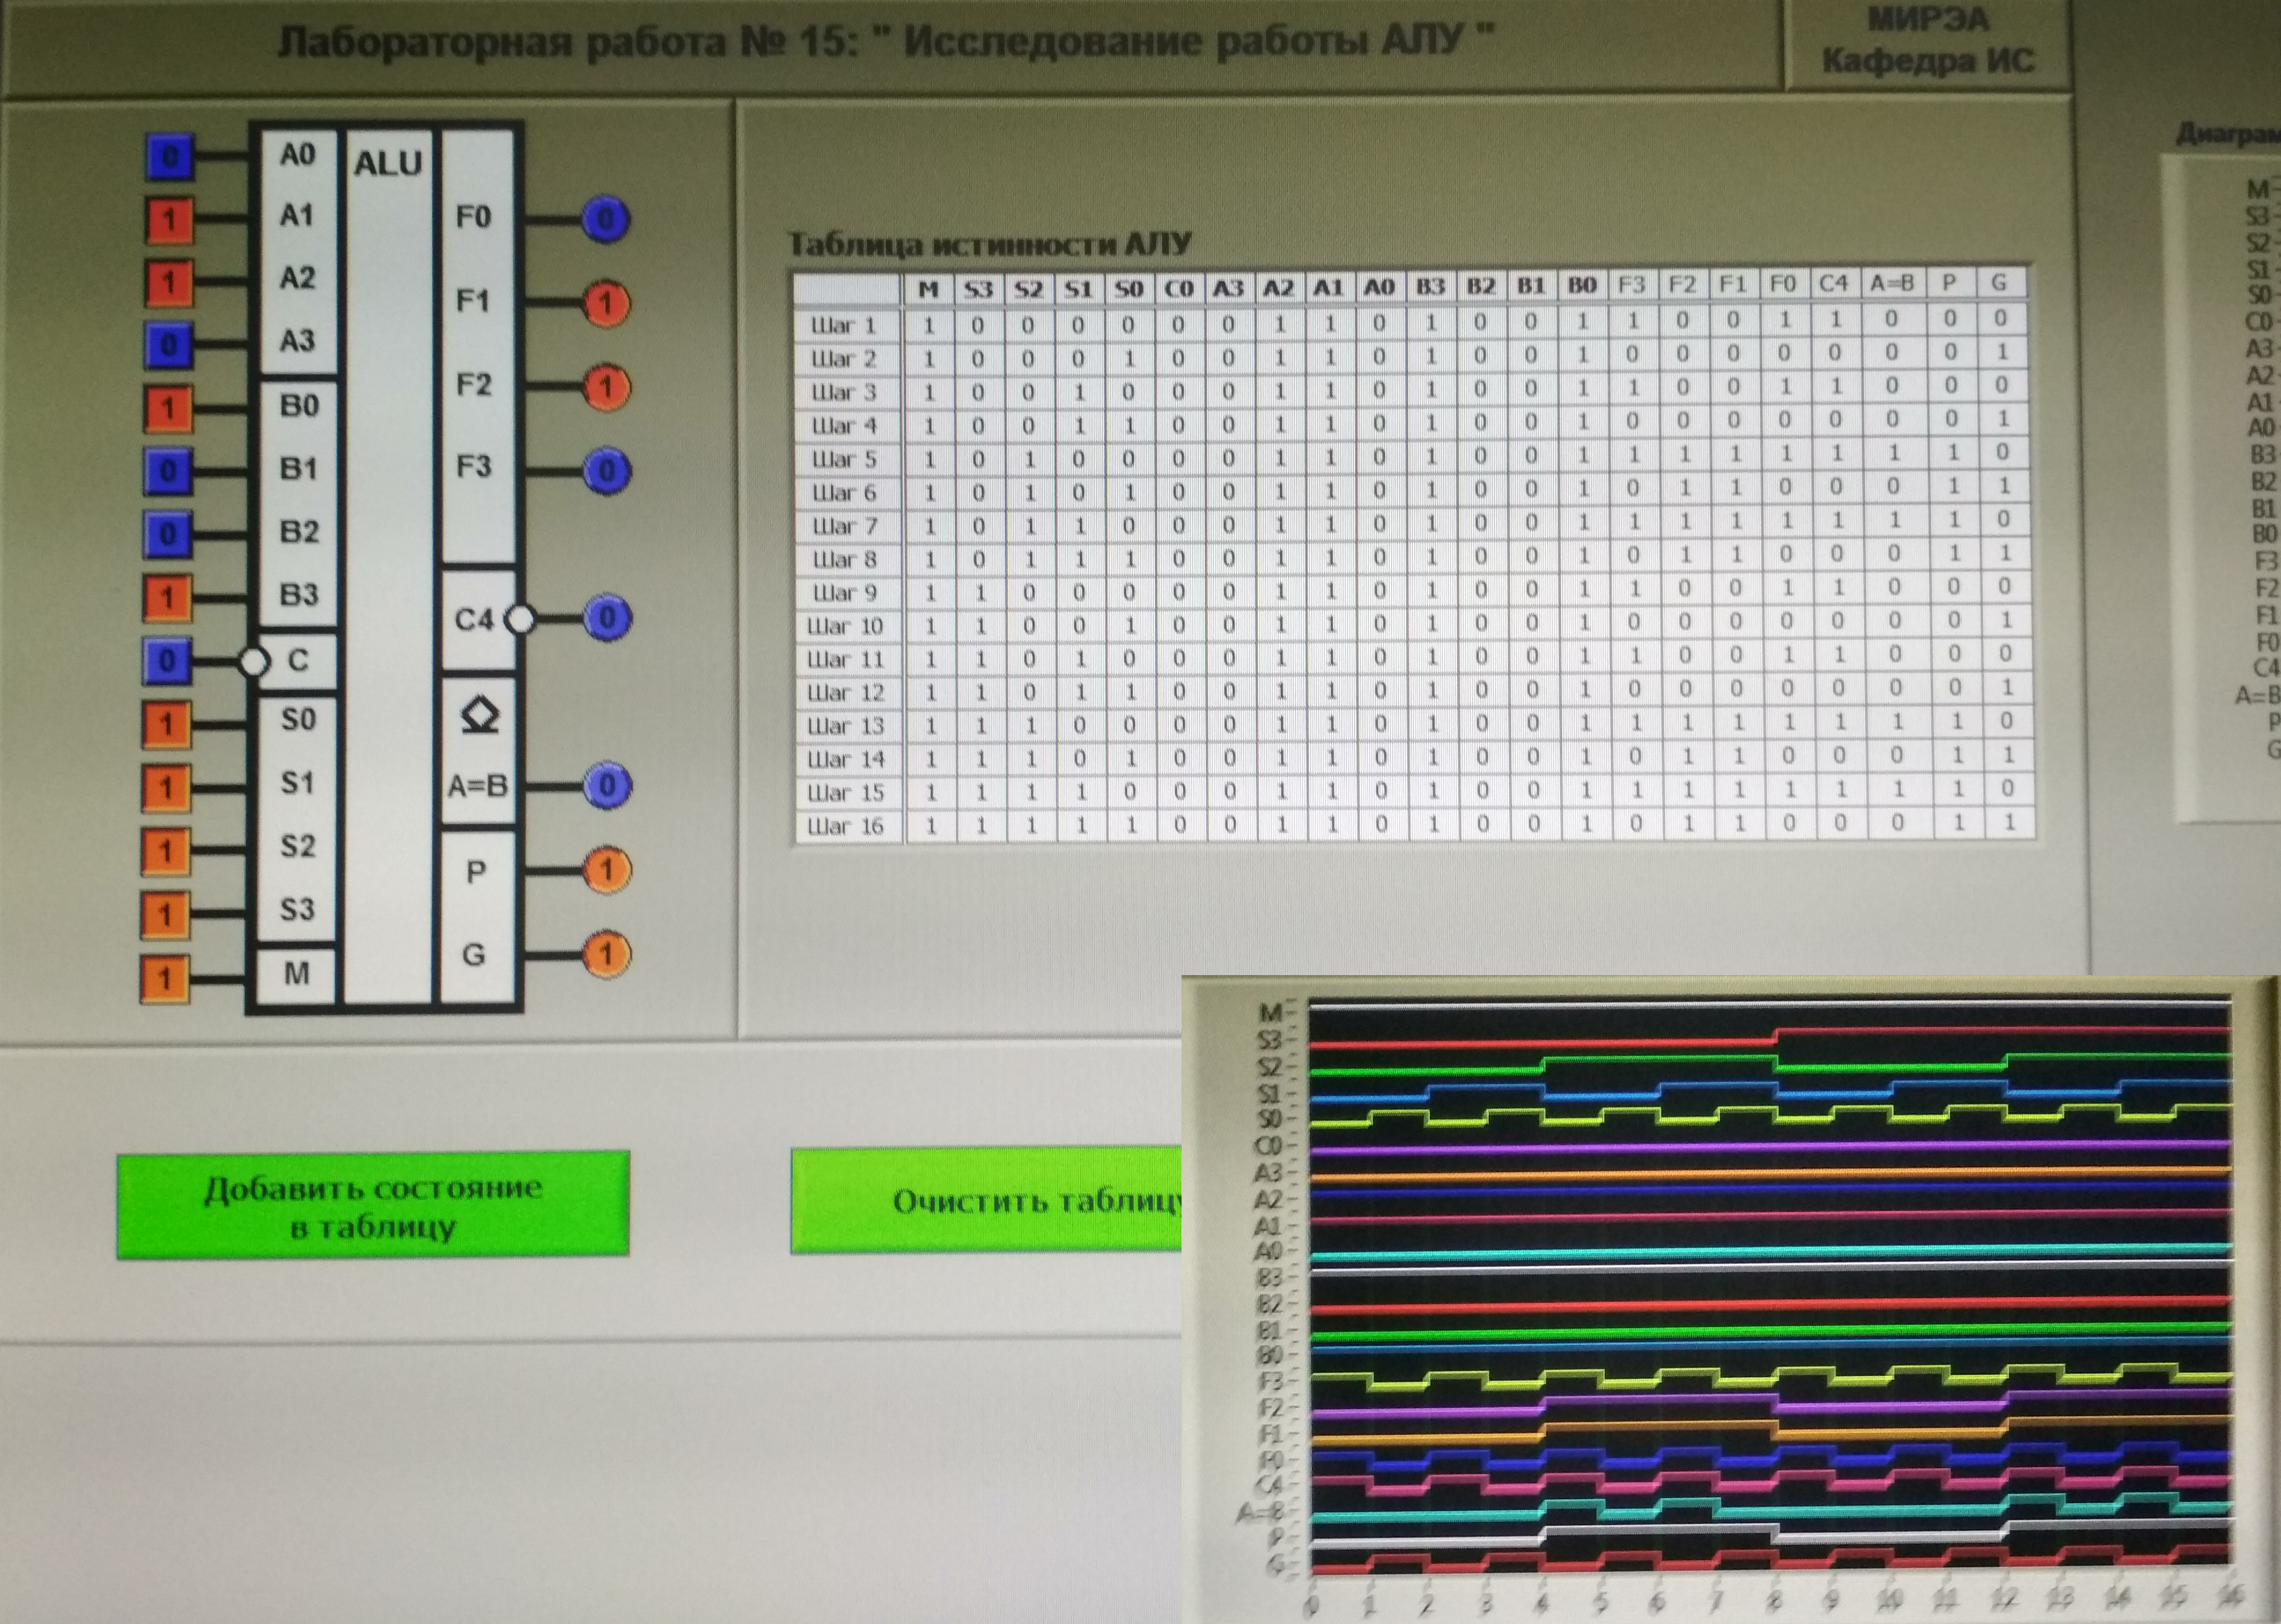
\includegraphics[width=0.95\linewidth]{imgs/14/1.jpg}
	\caption{РЕЖИМ СЧЕТА НА УВЕЛИЧЕНИЕ}
	\label{fig:14_1}
\end{figure}

\begin{figure}[H]
	\centering
	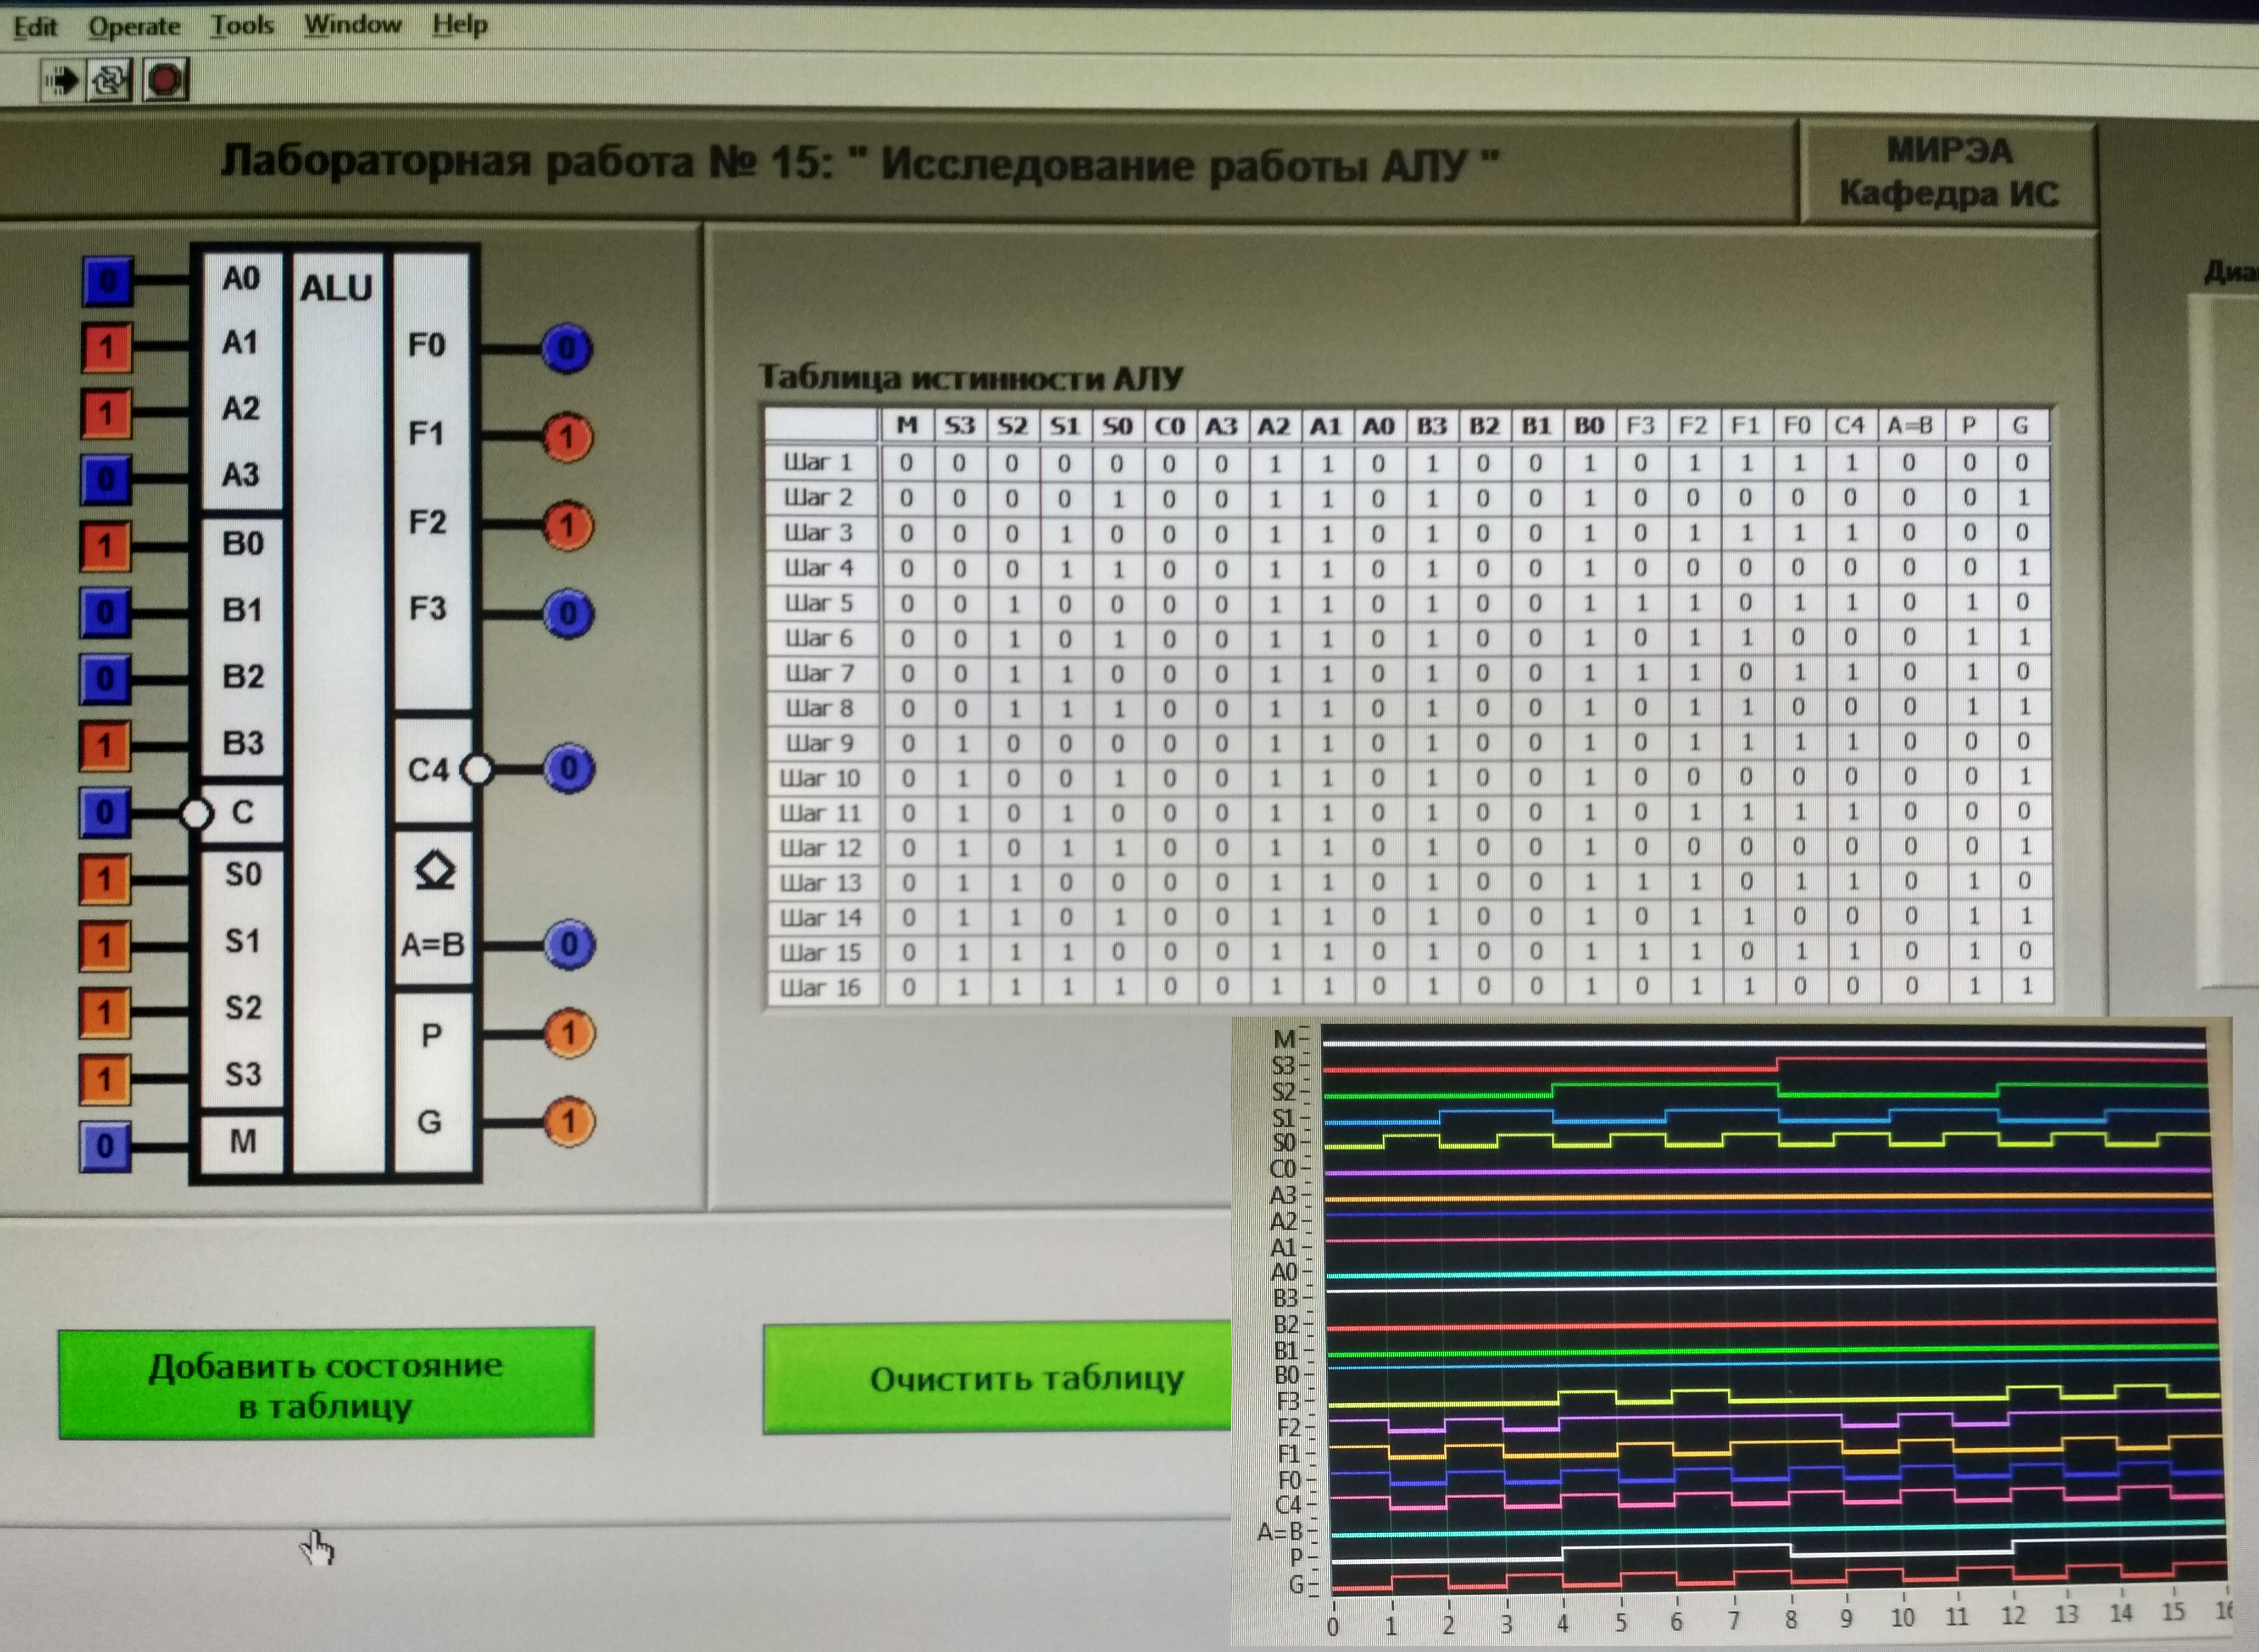
\includegraphics[width=0.95\linewidth]{imgs/14/2.jpg}
	\caption{РЕЖИМ СЧЕТА НА УМЕНЬШЕНИЕ}
	\label{fig:14_2}
\end{figure}

\begin{figure}[H]
	\centering
	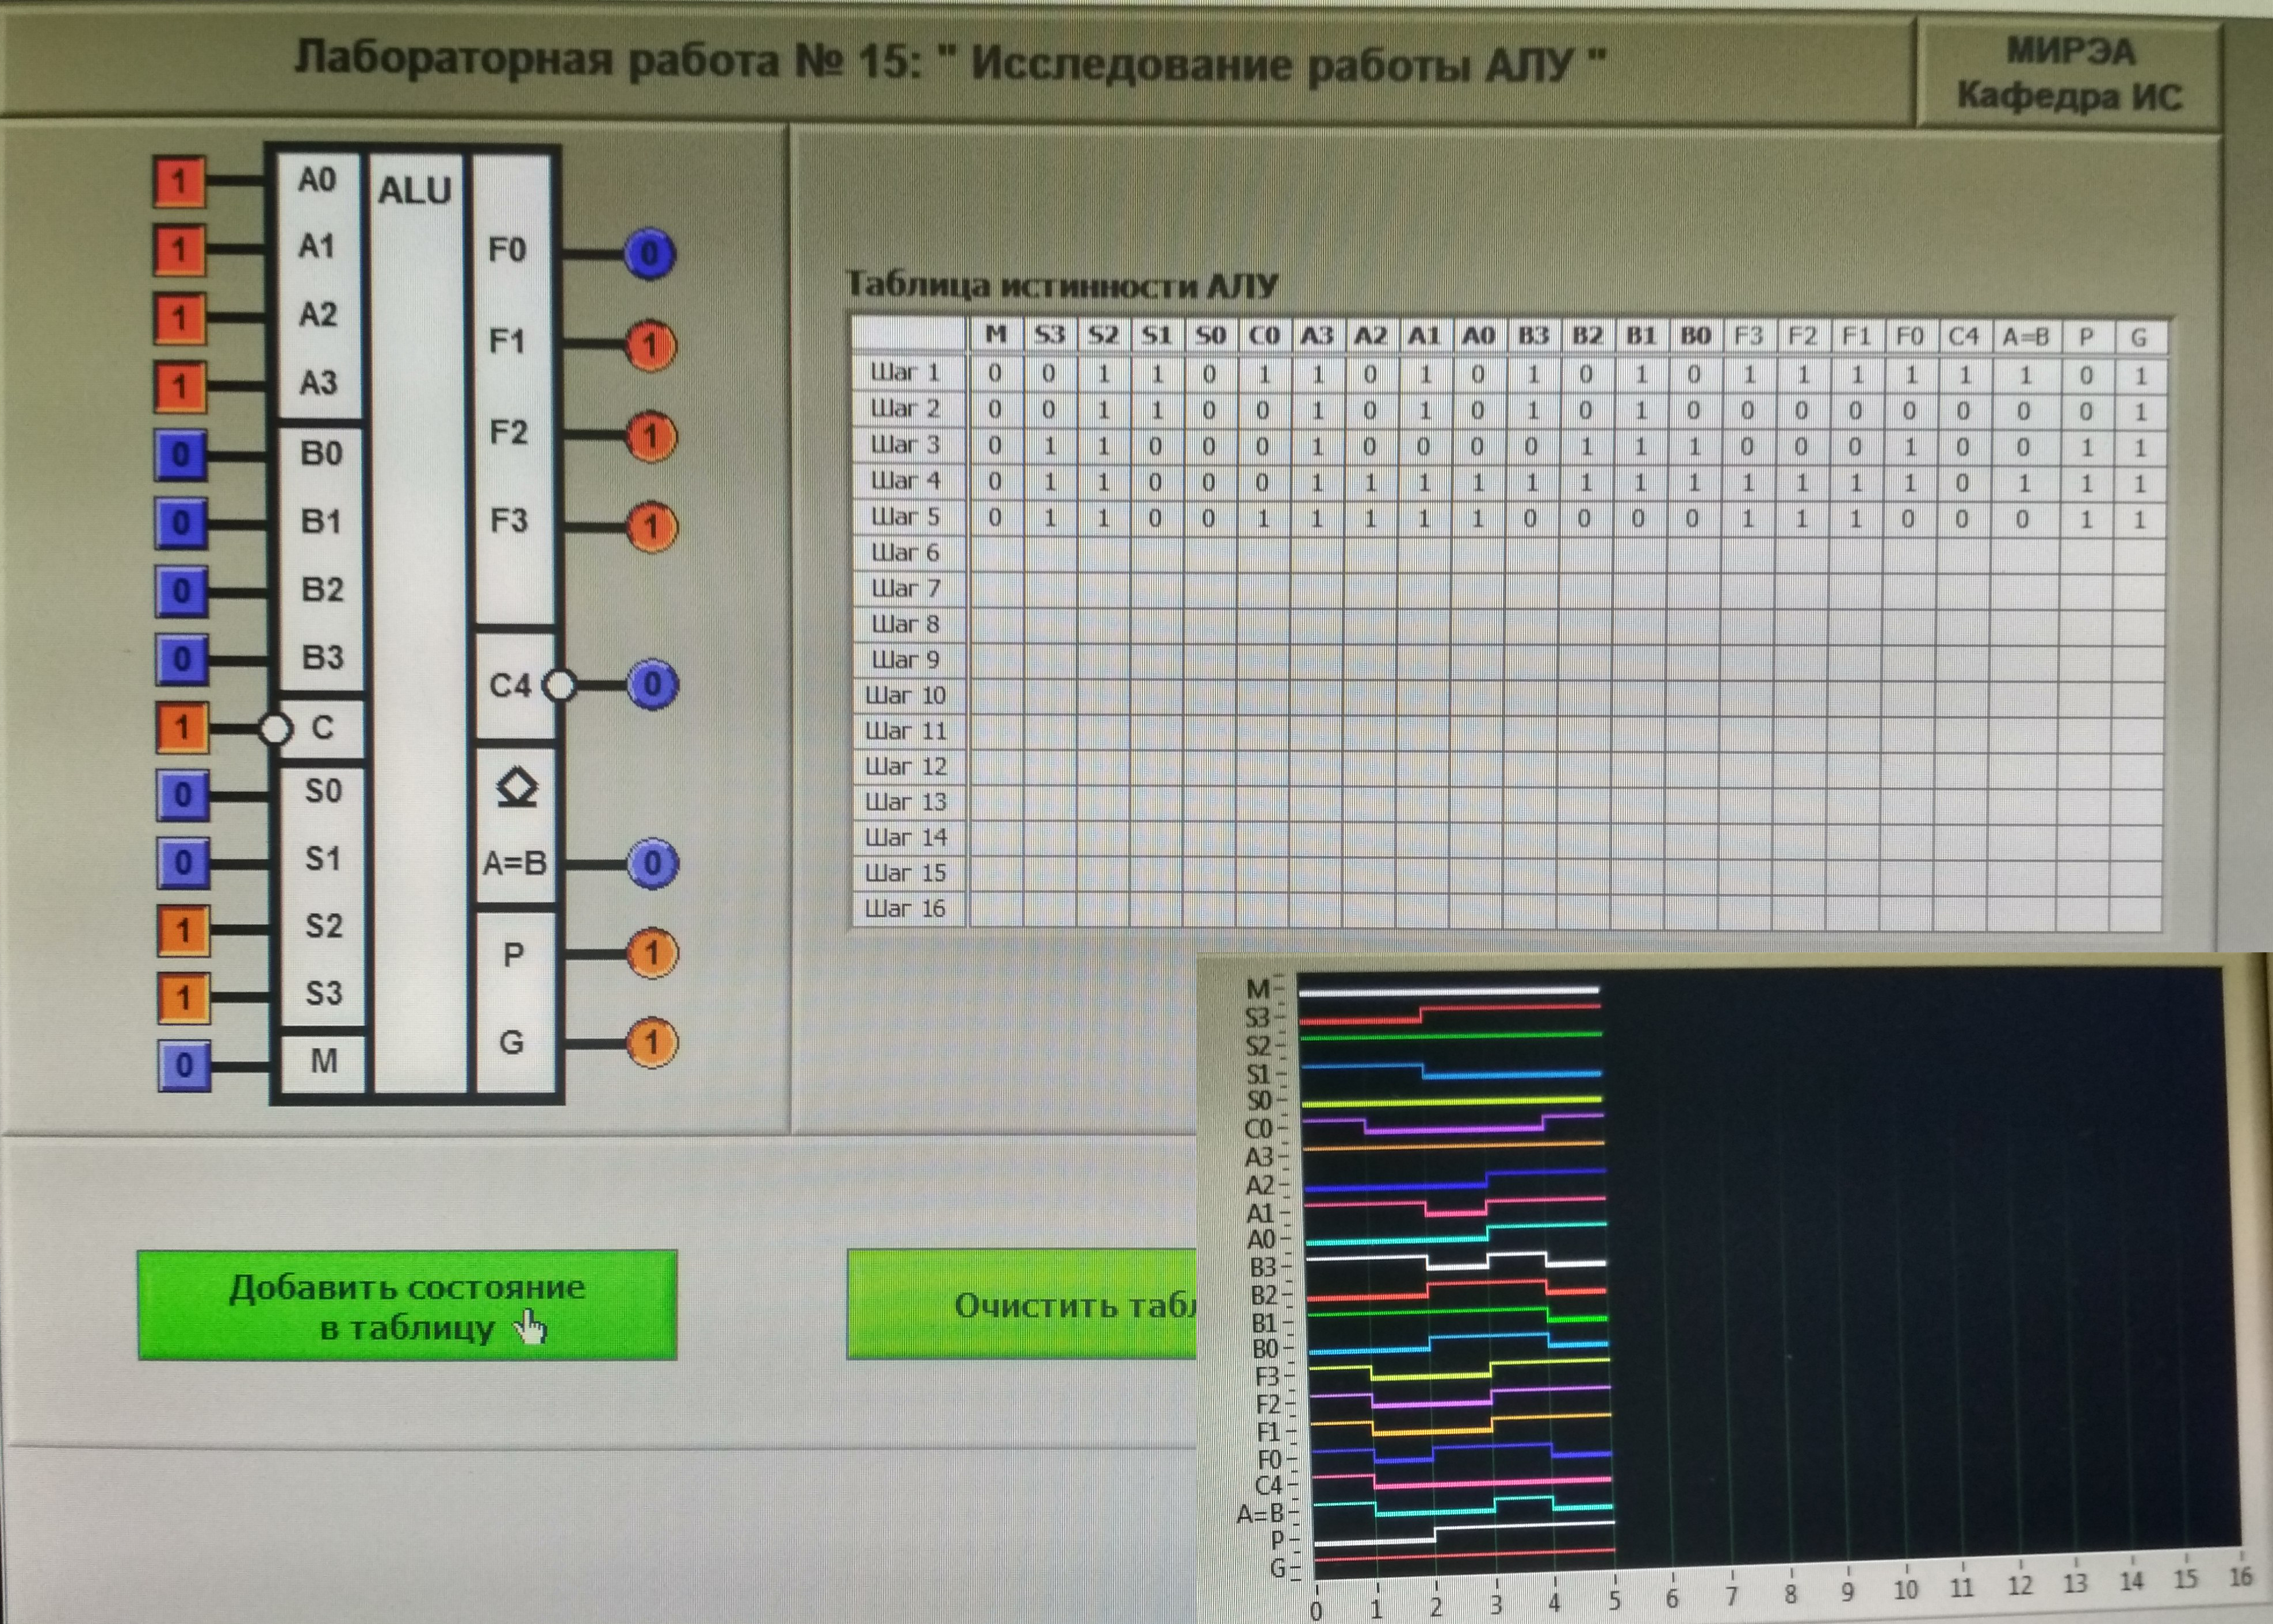
\includegraphics[width=0.95\linewidth]{imgs/14/3.jpg}
	\caption{РЕЖИМ ПАРАЛЛЕЛЬНОЙ ЗАГРУЗКИ}
	\label{fig:14_3}
\end{figure}

\begin{figure}[H]
	\centering
	\includegraphics[width=0.85\linewidth]{imgs/14/14_tab}
	\caption{Режим работы сумматора}
	\label{fig:14_tab}
\end{figure}

Элемент SN74LS193 

Характеристики:

\begin{figure}[H]
	\centering
	\includegraphics[width=0.95\linewidth]{imgs/14/14_sh}
	\caption{Схема}
	\label{fig:14_sh}
\end{figure}

\begin{figure}[H]
	\centering
	\includegraphics[width=0.8\linewidth]{imgs/14/14_rec}
	\caption{Рекомендуемые параметры}
	\label{fig:14_rec}
\end{figure}

\begin{figure}[H]
	\centering
	\includegraphics[width=0.95\linewidth]{imgs/14/14_ch}
	\caption{Электрические характеристики}
	\label{fig:14_ch}
\end{figure}

\begin{figure}[H]
	\centering
	\includegraphics[width=0.95\linewidth]{imgs/14/14_switch}
	\caption{Коммутационные характеристики}
	\label{fig:14_switch}
\end{figure}
